\documentclass[10pt,a4paper]{article}
\usepackage[utf8]{inputenc}
\usepackage{amsmath}
\usepackage{caption}
% Thing for images
\usepackage{graphicx}
\graphicspath{C:/Users/steve/Pictures/}
\usepackage{amsfonts}
\usepackage{amssymb}
% This sets the margin to look somewhat normal
\usepackage[margin=1in]{geometry}
\author{Steven Maio}
\title{Metro Map Maker Sofware Design Description}
\begin{document}

%%%%%%%%%%%%%%%%%%%%%%%
%% Table of contents %%
%%%%%%%%%%%%%%%%%%%%%%%
\tableofcontents

\newpage

% This makes sure that the spacing starts to the left
\flushleft

 \section{Introduction}
This is the Software Design Description (SDD) for the Metro Map Maker application.

\subsection{Purpose}
This document will serve as the blueprint for the construction of the Metro Map maker application. This document will use UML class diagrams to provide detail regarding packages, classes, instance variables, class variables, and method signatures needed for the application. In addition, UML Sequence diagrams will be used to specify object interactions post-initialization of the application, meaning in response to user interactions or timed events.

\subsection{Scope}
The Metro Map Maker will be a desktop application that will be built from the Desktop Java Framework (DJF). 

\subsection{Definitions, acronyms, and abbreviations}
\textbf{Class Diagram} - A UML document format that describes classes graphically. Specifically, it describes their instance variables, method headers, and relationships to other classes. \newline

\textbf{Framework} - In an object-oriented language, a collection of classes and interfaces that collectively provide a service for building applications or additional frameworks all with a common need. \newline

\textbf{Java} – A high-level programming language that uses a virtual machine layer between the Java application and the hardware to provide program portability. \newline

\textbf{Sequence Diagram} - A UML document format that specifies how object methods interact with one another. \newline

\textbf{UML} - Unified Modeling Language, a standard set of document formats for designing software graphically. \newline

\textbf{Desktop Java Framework (djf)} - The framework that the Metro Map Maker application will be built using.

\subsection{References}
\textbf{Metro Map Maker SRS} - Software requirements specification for the Metro Map Maker software application.

\subsection{Overview}
This Software Design Description document provides a design for the Metro Map Maker software application described in the Metro Map Maker SRS. The Java API being used to create the application are described in section 2, as well as their purpose. Section 3 provides an overview of the class design for the Metro Map Maker. Section 4 contains information on the use cases the program has been required. Section 5 contains information on how the program will store data. Section 6 contains supplementary information that may be useful to the reader. Note that all of the UML Diagrams used in this document were created in the VioletUML editor. \newpage

% Section 2 -- Package-Level Design Viewpoint
\section{Package-Level Design Viewpoint}
This application will be designed using the DJF. The software will also use Java API.

\subsection{Metro Map Maker overview}
The Metro Map Maker will use the following components directly from the DJF. These classes will not be discussed in detail in this document. \newline

\begin{center}
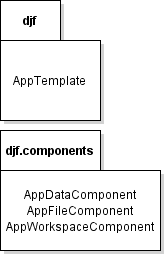
\includegraphics{DesktopJavaFramework_API.jpg}
\captionof{figure}{djf Framework directly used}
\end{center}

\subsection{Java API Usage}
The design for the Metro Map Maker will make use of the following classes specified in the following figure

\begin{center}
\includegraphics[scale=0.75]{/Users/steve/Pictures/hw3/classes/JavaAPI.png}
\captionof{figure}{The Java API being used}
\end{center}

% Here we'll descrie how the Java API is being used
\subsection{Java API Usage Descriptions}

% This is the section for the java.util package
\begin{center}
\begin{tabular}{| l | p{12cm} |}
\hline
Class/Interface & Use \\ \hline
File & This will be used for importing and exporting saved data for the Metro Map Maker, as well as importing images into a map \\ \hline
ArrayList & This class will be used to store groups of Data\\ \hline
LinkedList & This class is used as the parent class of the MetroLine class. This seemed appropriate as a Metro Line would be an ordered collection with a designated head and tail. \\ \hline
\end{tabular}
\captionof{table}{Uses for the classes in the Java API's java.util package}
\end{center}

% This section is for the java.scene.shape package
\begin{center}
\begin{tabular}{| l | p{12cm} |}
\hline
Class/Interface & Use \\ \hline
Line & This class will be used to draw the connections between Metro Stations on the map \\ \hline
Circle & This class is used to indicate on the map where the Metro Stations are located \\ \hline
Rectangle & This class is used to allow for the user to add images to the metro map they are editing \\ \hline
\end{tabular}
\captionof{table}{Uses for the classes in the Java API's javafx.scene.shape package}
\end{center}

% This is the section for the javafx.collections package
\begin{center}
\begin{tabular}{| l | p{12cm} |}
\hline
Class/Interface & Use \\ \hline
ObservableList & This class is used to allow for MMMData and MMMWorkspace to interact with each other fairly well. \\ \hline
\end{tabular}
\captionof{table}{Uses for the classes in the Java API's javafx.collections package}
\end{center}

% This is for javafx.scene.image
\begin{center}
\begin{tabular}{| l | p{12cm} |}
\hline
Class/Interface & Use \\ \hline
Image & This class will be used to add images to the metro map being edited, as well adding an image background to a map\\ \hline
\end{tabular}
\captionof{table}{Uses for the classes in the Java API's javafx.scene.image package}
\end{center}

% javafx.scene.text
\begin{center}
\begin{tabular}{| l | p{12cm} |}
\hline
Class/Interface & Use \\ \hline
Text & This class will be extended so that the user will be able to add labels to the metro map being edited \\ \hline
\end{tabular}
\captionof{table}{Uses for the classes in the Java API's javafx.scene.text package}
\end{center}

% javafx.scene.paint
\begin{center}
\begin{tabular}{| l | p{12cm} |}
\hline
Class/Interface & Use \\ \hline
Color & This class will be used to change the fill color of shapes on the metro map, as well as set the background color. \\ \hline
ImagePattern & This class is used in the scenario where the user wishes to add an image to the map being edited \\ \hline
\end{tabular}
\captionof{table}{Uses for the classes in the Java API's javafx.scene.paint package}
\end{center}

% javafx.stage
\begin{center}
\begin{tabular}{| l | p{12cm} |}
\hline
Class/Interface & Use \\ \hline
Stage & This class will be extended for all of the dialog windows which are outside of the main editor. This includes the WelcomeDialog, EnterTextDialog, etc. \\ \hline
\end{tabular}
\captionof{table}{Uses for the classes in the Java API's javafx.stage package}
\end{center}

% javafx.scene.control
\begin{center}
\begin{tabular}{| l | p{12cm} |}
\hline
Class/Interface & Use \\ \hline
Label & This class is used to label windows, and other objects in the GUI \\ \hline
Button & This class is used frequently and it provides the user with many options to control and edit their metro map \\ \hline
ComboBox & This class is used to allow the user to select certain types of data. \\ \hline
ColorPicker & This class is used to offer to the user a large variety of colors to use as the fill for shapes on the metro map or for the background color \\ \hline
Slider & This class will allow the user to have a finer control over the selection of certain variables in the application. \\ \hline
CheckBox & This class will be used to allow the user to set certain editing options which only have two options available \\ \hline
\end{tabular}
\captionof{table}{Uses for the classes in the Java API's javafx.scene.control package}
\end{center}

% javafx.scene.layout
\begin{center}
\begin{tabular}{| l | p{12cm} |}
\hline
Class/Interface & Use \\ \hline
Pane & The main container for all the objects in a metro map \\ \hline
FlowPane & This container is used so to automatically organize certain toolbars in the main window \\ \hline
HBox & This class will be used as the main container for all of the toolbars in the editor \\ \hline
GridPane & This will be used as the container for certain toolbars \\ \hline
\end{tabular}
\captionof{table}{Uses for the classes in the javafx.scene.layout package}
\end{center}

\section{Class-Level Design Viewpoint}
As stated before, the design will encompass the Metro Map Maker application and Desktop Java Framework. Since no modifications are being made to the Desktop Java Framework, the UML documentation for the Desktop Java Framework will not be provided. For the purpose of fitting all the diagrams to the pages, the diagrams will be split up.


\begin{center}
\includegraphics{C:/Users/steve/Pictures/hw3/Draggable.jpg}
\captionof{figure}{Draggable}
\end{center}

\begin{center}
\includegraphics{C:/Users/steve/Pictures/hw3/BorderedMessageDialog.jpg}
\captionof{figure}{BorderedMessageDialog}
\end{center}

\begin{center}
\includegraphics{C:/Users/steve/Pictures/hw3/DraggableImage.jpg}
\captionof{figure}{DraggableImage}
\end{center}

\begin{center}
\includegraphics{C:/Users/steve/Pictures/hw3/DraggableLabel.jpg}
\captionof{figure}{DraggableLabel}
\end{center}

\begin{center}
\includegraphics{C:/Users/steve/Pictures/hw3/EnterTextDialog.jpg}
\captionof{figure}{EnterTextDialog}
\end{center}

\begin{center}
\includegraphics{C:/Users/steve/Pictures/hw3/MetroLine_and_Node.jpg}
\captionof{figure}{MetroLine and MetroLineNode classes}
\end{center}

\begin{center}
\includegraphics{C:/Users/steve/Pictures/hw3/MetroLineSettingsDialog.png}
\captionof{figure}{MetroLineSettingsDialog}
\end{center}

\begin{center}
\includegraphics{C:/Users/steve/Pictures/hw3/MetroStation.jpg}
\captionof{figure}{MetroStation}
\end{center}

\begin{center}
\includegraphics{C:/Users/steve/Pictures/hw3/MMMApp.jpg}
\captionof{figure}{MMMApp}
\end{center}

\begin{center}
\includegraphics{C:/Users/steve/Pictures/hw3/MMMCanvasController.jpg}
\captionof{figure}{MMMCanvasController}
\end{center}

\begin{center}
\includegraphics[scale=.75]{C:/Users/steve/Pictures/hw3/classes/MMMData.jpg}
\captionof{figure}{MMMData}
\end{center}

\begin{center}
\includegraphics{C:/Users/steve/Pictures/hw3/MMMEditController.jpg}
\captionof{figure}{MMMEditController}
\end{center}

\begin{center}
\includegraphics{C:/Users/steve/Pictures/hw3/MMMState.jpg}
\captionof{figure}{MMMState Enum}
\end{center}

\begin{center}
\includegraphics[scale=0.9]{C:/Users/steve/Pictures/hw3/MMMWorkspace.jpg}
\captionof{figure}{MMMWorkspace}
\end{center}

\begin{center}
\includegraphics{C:/Users/steve/Pictures/hw3/WelcomeDialog.jpg}
\captionof{figure}{WelcomeDialog}
\end{center}

\newpage

% Section 4
\section{Method Level Design Viewpoint}
The following diagrams will describe the methods that will be called within the code.

\begin{center}
\includegraphics[scale=0.6]{C:/Users/steve/Pictures/hw3/use_cases/2_1.png}
\captionof{figure}{Create new map from the Welcome Dialog}
\end{center}

\begin{center}
\includegraphics[scale=0.7]{C:/Users/steve/Pictures/hw3/use_cases/2_2.png}
\captionof{figure}{Select Recent Map to Load}
\end{center}

\begin{center}
\includegraphics[scale=0.7]{C:/Users/steve/Pictures/hw3/use_cases/2_3.png}
\captionof{figure}{Close Welcome Dialog}
\end{center}

\begin{center}
\includegraphics[scale=0.5]{C:/Users/steve/Pictures/hw3/use_cases/2_9.png}
\captionof{figure}{Undo Edit}
\end{center}

\begin{center}
\includegraphics[scale=0.7]{C:/Users/steve/Pictures/hw3/use_cases/2_10.png}
\captionof{figure}{Redo Edit}
\end{center}

\begin{center}
\includegraphics[scale=0.7]{C:/Users/steve/Pictures/hw3/use_cases/2_11.png}
\captionof{figure}{Learn About Application}
\end{center}

\begin{center}
\includegraphics[scale=0.6]{C:/Users/steve/Pictures/hw3/use_cases/2_13.png}
\captionof{figure}{Remove Metro Line}
\end{center}

\begin{center}
\includegraphics[scale=0.5]{C:/Users/steve/Pictures/hw3/use_cases/2_14.png}
\captionof{figure}{Edit Line}
\end{center}

\begin{center}
\includegraphics[scale=0.65]{C:/Users/steve/Pictures/hw3/use_cases/2_15.png}
\captionof{figure}{Move Line end points}
\end{center}

\begin{center}
\includegraphics[scale=0.6]{C:/Users/steve/Pictures/hw3/use_cases/2_16a.png}
\captionof{figure}{Add Stations to Line - Entering Add Stations Mode.}
\end{center}

\begin{center}
\includegraphics[scale=0.6]{C:/Users/steve/Pictures/hw3/use_cases/2_16b.png}
\captionof{figure}{Add Stations to Line - Adding stations to a Metro Line.}
\end{center}

\begin{center}
\includegraphics[scale=0.6]{C:/Users/steve/Pictures/hw3/use_cases/2_16c.png}
\captionof{figure}{Add Stations to Line - Exiting Add Stations Mode.}
\end{center}

\begin{center}
\includegraphics[scale=0.5]{C:/Users/steve/Pictures/hw3/use_cases/2_17a.png}
\captionof{figure}{Remove Stations - Entering Remove Stations Mode}
\end{center}

\begin{center}
\includegraphics[scale=0.5]{C:/Users/steve/Pictures/hw3/use_cases/2_17b.png}
\captionof{figure}{Remove Stations - Removing Stations and Exiting Remove Stations Mode.}
\end{center}

\begin{center}
\includegraphics[scale=0.5]{C:/Users/steve/Pictures/hw3/use_cases/2_20.png}
\captionof{figure}{Add New Station}
\end{center}

\begin{center}
\includegraphics[scale=0.5]{C:/Users/steve/Pictures/hw3/use_cases/2_23.png}
\captionof{figure}{Move Station Label}
\end{center}

\newpage

% Section 5
\section{File Structure and Formats}
The Desktop Java Framework will be provided inside the MetroMapMaker.jar. This needs to be imported into the necessary project for the Metro Map Maker application.
\subsection{Application Data}
Various forms of data will be kept for the Metro Map Maker. We will have various language properties (stored in an .xml file) stored inside the data folder along with a schema. \linebreak

Images will be stored in an image folder for ease of access.

% Section 6.1
\subsection{Exporting Data}
A Metro Map Maker file will be saved using the JSON strucutre. For each map the following data fields are saved: \linebreak

% Map Data
\textbf{Map}
\begin{itemize}
\item Background Color
\item Background Image (If one is chosen)
\end{itemize}

% Metro Station Data
\textbf{Metro Station}
\begin{itemize}
\item Name
\item X-Coordinate
\item Y-Coordinate
\item Fill Color
\item Radius
\item Label Rotation
\item Label Position
\end{itemize}

% Metro Line Data
\textbf{Metro Line}
\begin{itemize}
\item Name
\item Fill Color
\item Line Thickness
\item Start Label X-Coordinate
\item Start Label Y-Coordinate
\item End Label X-Coordinate
\item End Label Y-Coordinate
\item Metro Station Stops
\end{itemize}

% Labels
\textbf{Labels}
\begin{itemize}
\item Text
\item X-Coordinate
\item Y-Coordinate
\item Bold Font
\item Italic Font
\item Font Family
\item Font Size
\item Font Fill
\end{itemize}

% Images
\textbf{Images}
\begin{itemize}
\item Image filepath
\item X-Coordinate
\item Y-Coordnate
\end{itemize}

% Section 6
\section{Supporting Information}
N/A
\end{document}
